\subsection{A stylized reading of the 2025 episode}
\label{sec:2025}

The 2025 exercise is neither a calibration nor a causal test. The model is static, has flexible prices, and is evaluated around balanced trade, while observed exchange rates are high-frequency asset prices affected by many contemporaneous shocks. We use the model only to classify the sign patterns associated with different tariff configurations. For each phase, we identify the tariff configuration, state the sign pattern associated with that configuration, compare it with the observed exchange-rate movements, and limit the inference to sign consistency.

Observed exchange-rate movements do not identify $\rho$, $\rho_D$, or the contribution of the trade mechanism. A movement is described as consistent with the model only when its sign matches the model's sign under the stated tariff configuration and parameter condition. \Cref{tab:phases} and \cref{fig:episode} report the data, with a positive number a depreciation of the dollar; the Federal Reserve's broad dollar index is the closest counterpart of the model's trade-weighted NEER, and the index excluding China isolates the bystanders.

\begin{table}[t]
\centering
\caption{Exchange-rate changes within the three phases of the 2025 episode (percent; positive = dollar depreciation)}
\label{tab:phases}
\small
\begin{tabular}{lcccccc}
\toprule
 & \multicolumn{2}{c}{Phase 1} & \multicolumn{2}{c}{Phase 2} & \multicolumn{2}{c}{Phase 3} \\
 & \multicolumn{2}{c}{Feb~1--Apr~2} & \multicolumn{2}{c}{Apr~3--May~12} & \multicolumn{2}{c}{Aug~7--Dec~31} \\
\cmidrule(lr){2-3}\cmidrule(lr){4-5}\cmidrule(lr){6-7}
 & Monthly & Daily & Monthly & Daily & Monthly & Daily \\
\midrule
\tabinput{tables/tab6_phases.tex}
\bottomrule
\end{tabular}

\vspace{4pt}
\begin{minipage}{0.95\textwidth}\footnotesize
\textit{Notes:} Monthly columns compare monthly averages (January with March, March with April, July with December); daily columns compare the last available observations at the phase boundaries (January~31 to April~2, April~2 to May~12, August~6 to December~31). VND daily entries (marked $^{a}$) use BIS end-of-month rates. Sources: Federal Reserve H.10 and BIS; see \cref{app:episode-data}.
\end{minipage}
\end{table}

\paragraph{Phase 1: China-focused escalation (February~1--April~2).} The United States raised tariffs on China, while China responded with narrower product-specific tariffs. The United States also imposed tariffs on Canada and Mexico, and Canada retaliated, so this phase is not a clean unilateral-tariff experiment. Approximating it as a tariff concentrated on China, \cref{prop:unilateral} associates the configuration with dollar appreciation against the target and, when $\rho>N\rho_D$, depreciation against untariffed bystanders. The dollar was approximately unchanged against the renminbi and weakened against the euro and the broad index excluding China. The bystander movements are consistent with the high-$\rho$ sign pattern, but the mixed tariff configuration and contemporaneous shocks prevent a sharper inference.

\begin{figure}[t]
\centering
\begin{subfigure}[t]{0.9\textwidth}\centering
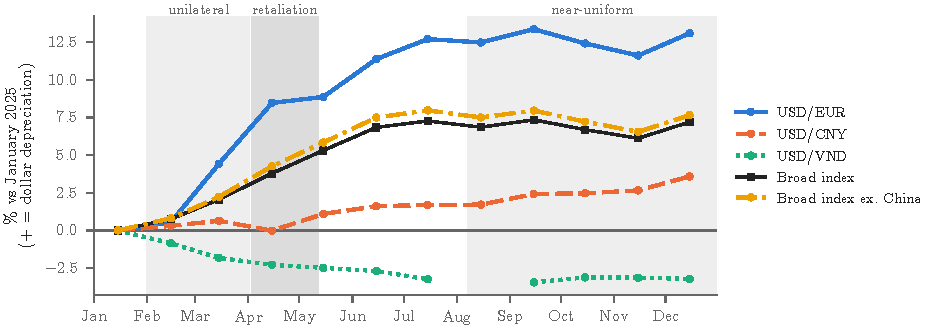
\includegraphics[width=\textwidth]{fig7a_fx2025.pdf}
\caption{Exchange rates, percent deviation from the January~2025 average (positive = dollar depreciation)}
\end{subfigure}

\vspace{6pt}
\begin{subfigure}[t]{0.9\textwidth}\centering
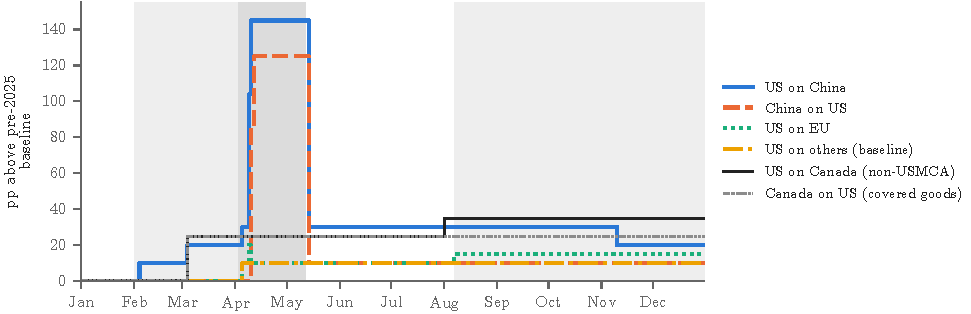
\includegraphics[width=\textwidth]{fig7b_tariffs2025.pdf}
\caption{Headline tariff increases above the pre-2025 baseline (percentage points)}
\end{subfigure}
\caption{Exchange rates and headline tariff increases during 2025. Shading denotes the three policy phases. Sources: Federal Reserve, BIS, Federal Register, Department of Finance Canada, and China's State Council Tariff Commission.}
\label{fig:episode}
\end{figure}

\paragraph{Phase 2: US--China retaliation (April~3--May~12).} The United States and China raised tariffs sharply against each other, while most other partners faced a common 10 percent US baseline tariff. The configuration is therefore closest to bilateral retaliation with an additional uniform component. \Cref{prop:retaliation} associates bilateral retaliation with a stable rate between the belligerents and, when $\rho>\rho_D$, depreciation against bystanders and in effective terms. During the phase, the dollar moved little against the renminbi but depreciated against the euro, the broad index excluding China, and the full broad index. This is the phase most closely aligned with the retaliation sign pattern. The comparison establishes sign consistency only; it does not identify the relevant elasticity or the contribution of the trade mechanism.

\paragraph{Phase 3: Near-uniform tariffs with residual retaliation (August~7--December~31).} US tariffs became more nearly uniform across partners, although higher rates and retaliation remained for some countries. The broader uniform component strengthens the average-protection channel, which pushes toward effective dollar appreciation, while the remaining discriminatory and retaliatory components can push in the opposite direction. The broad dollar index was approximately flat within the phase, with no clear effective appreciation. Over 2025 as a whole, the dollar depreciated substantially, by $7.2$ percent against the broad index and $7.6$ percent against the index excluding China between the January and December monthly averages, with most of that movement occurring before August. The static trade mechanism therefore does not account for the full effective depreciation. A quantitative assessment would require the complete tariff network, substitution elasticities, trade weights, retaliation, and a dynamic mechanism linking expected policy to asset prices.

The comparison across phases is more informative than any individual episode. A configuration dominated by bilateral retaliation is associated with stronger bystander and effective depreciation forces, while broader uniform protection strengthens the average-protection force. The observed movements in Phase~2 have the sign pattern associated with retaliation, whereas Phase~3 provides no corresponding broad appreciation as protection became more uniform. These comparisons illustrate the importance of the tariff configuration without identifying tariffs as the cause of the exchange-rate movements.

\FloatBarrier
